% =======================================================================================
\section{Dividing the Band}
\label{sec:narrow-band}
% =======================================================================================
% Rewritten 2026-11-19 (user): the response width R sets the highest frequency kept with high
% fidelity and the tensor shapes, so the band is split into bands of one R each, trained one per
% device; four bands by R alone (32, 64, 128, more); the visible sources sit in the R = 64 band,
% which is the narrow band, trained on one device as a simplified scenario; the full band is one
% device over the whole band at R = 128, a scalability check rather than the intended scheme.
% Numbers from paper/scripts/numbers_narrow-band.py (reports/prior/response-span). Labels kept:
% sec:narrow-band-span, sec:narrow-band-prior, sec:narrow-band-bands, tab:forward-model-bands.

\paragraph{How many bins a response needs.}
\label{sec:narrow-band-span}
Each source enters its window as a response of $R$ frequency bins around $f_0\Tobs$
(\cref{sec:gw-windows}). The response spreads over the annual Doppler sideband, which grows in
proportion to $f_0$, the chirp drift $\fdot\,\Tobs$, which grows as $f_0^{11/3}$ at a given chirp
mass (\cref{eq:forward-model-fdot}), and the sidebands of the antenna pattern, which do not depend
on $f_0$ (\cref{eq:forward-model-span}). Bounding these terms for every source the prior allows
takes $R=\ForwardModelSpanBound$ at the top of the band, but most of those bins lie below the noise.
What matters is the power the data can see: per bin, the signal power in excess of the noise's. We
therefore size $R$ by a fuzzy bound, the smallest power of two that keeps a share $x$ of a source's
above-noise power for a share $y$ of the sources that have any (\cref{app:forward-model-heterodyne}).
The median such source needs \ForwardModelSpanMedian{} bins, and $R=\ForwardModelSpanNeedAll$ keeps
every above-noise bin of \qty{99.9}{\percent} of them over the whole band. The need grows with
frequency: keeping every above-noise bin of \qty{\NarrowBandSharePercent}{\percent} of the sources
at a given $f_0$ takes $R=\NarrowBandOneR$ up to \qty{\NarrowBandOneHighMhz}{\milli\hertz},
\NarrowBandTwoR{} up to \qty{\NarrowBandTwoHighMhz}{\milli\hertz}, \NarrowBandThreeR{} up to
\qty{\NarrowBandThreeHighMhz}{\milli\hertz} and \NarrowBandTopR{} at
\qty{\NarrowBandFourHighMhz}{\milli\hertz}. Choosing $R$ thus chooses the highest frequency whose
sources are represented with high fidelity and high probability (\cref{fig:narrow-band}a).

\paragraph{One band per device.}
$R$ fixes the shapes of every tensor: a window holds $K=\ForwardModelWindowResponses{}R$ bins, and
its tokens follow. A single $R$ must suit the top of the band, and is then far too wide at the
bottom, where a window of \RatesFullWindow{} bins holds up to \num{\RatesFullAllHi} sources of the
catalogue (\cref{sec:gw-rates}). We therefore divide the band and conquer each part separately:
training runs on several devices, each simulating and processing the windows of its own band at
that band's $R$, and the gradients of one network are summed across devices. Every batch is then
stratified over the whole spectrum by construction. How many bands to use and how wide to make them
depends on $R$, and also on how many visible sources a window holds at each frequency, which sets
the number of sources $S$ the flow must resolve. We let $R$ alone decide, and cut the band where it
doubles, into the four bands of \cref{tab:narrow-band-bands}.

\begin{table}[t]
\caption{The band divided where the response width doubles: the $R$ that keeps every above-noise
bin of \qty{\NarrowBandSharePercent}{\percent} of the sources at each $f_0$, and each band's share of
the catalogue's sources and of the visible ones ($\snr\ge\NarrowBandVisibleSnr$).}
\label{tab:narrow-band-bands}
\centering
\small
\setlength{\tabcolsep}{4pt}
\begin{tabular}{@{}crrr@{}}
\toprule
$f_0$ [mHz] & $R$ & catalogue [\%] & visible [\%] \\
\midrule
\numrange{\NarrowBandOneLowMhz}{\NarrowBandOneHighMhz} & \NarrowBandOneR & \NarrowBandOneCatalogue & \NarrowBandOneVisible \\
\numrange{\NarrowBandTwoLowMhz}{\NarrowBandTwoHighMhz} & \NarrowBandTwoR & \NarrowBandTwoCatalogue & \NarrowBandTwoVisible \\
\numrange{\NarrowBandThreeLowMhz}{\NarrowBandThreeHighMhz} & \NarrowBandThreeR & \NarrowBandThreeCatalogue & \NarrowBandThreeVisible \\
\numrange{\NarrowBandFourLowMhz}{\NarrowBandFourHighMhz} & \numrange{256}{\NarrowBandTopR} & \NarrowBandFourCatalogue & \NarrowBandFourVisible \\
\bottomrule
\end{tabular}
\end{table}

\begin{figure}[t]
  \centering
  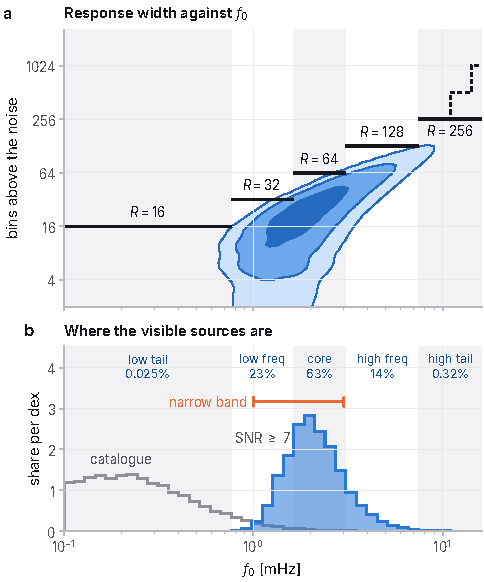
\includegraphics[width=\columnwidth]{figures/narrow-band.pdf}
  \caption{The band divided where the response width doubles (shaded and white strips;
  \cref{tab:narrow-band-bands}). (a)~Sources with power above the noise, by $f_0$ and by the bins
  that hold all of it; contours hold \qtylist{50;90;99}{\percent} of them. Lines: each band's $R$,
  which keeps every above-noise bin of \qty{\NarrowBandSharePercent}{\percent} of the sources at each
  $f_0$; in the top band that $R$ (dashed) climbs to \NarrowBandTopR{}. (b)~Share per dex of $f_0$
  of the catalogue's sources (grey) and of the visible ones, $\snr\ge\NarrowBandVisibleSnr$ (blue),
  with each band's share of the visible ones, and the narrow band (orange).}
  \label{fig:narrow-band}
\end{figure}

\paragraph{Where the visible sources are.}
\label{sec:narrow-band-prior}
The catalogue puts almost all its sources in the lowest band, where they are faint: the
conditional mean amplitude reaches that of a source at $\snr=\PriorsVisibleSnr$ only above
\qty{\PriorsAmpCrossMhz}{\milli\hertz} (\cref{fig:priors}e). The visible sources are its loud tail,
and \qty{\NarrowBandTwoVisible}{\percent} of them fall in the second band, at $R=\NarrowBandTwoR$
(\cref{tab:narrow-band-bands}, \cref{fig:narrow-band}b). Even within a band, windows centred on the catalogue's $f_0$
marginal would mostly hold no visible source, so training places its windows by
\cref{eq:priors-window}, with weight the catalogue's $f_0$ marginal times the chance that a source
there is visible, and \qty{\PriorsUniformWindowsPercent}{\percent} of them log-uniformly
(\cref{fig:priors}d, \cref{app:priors-window}). The weights choose which windows training sees, not
what their sources are, so the posterior given a window is unchanged.

\paragraph{The narrow band.}
\label{sec:narrow-band-bands}
We study the band that holds the bulk of the visible sources as a simplified scenario: one device,
one band, $R=\ForwardModelNarrowR{}$. The narrow band runs from
\qtyrange{\PriorsNarrowLowMhz}{\PriorsNarrowHighMhz}{\milli\hertz}, its lower edge taken down into
the first band, whose sources $R=\ForwardModelNarrowR$ holds with room to spare; it holds
\qty{\NarrowBandNarrowVisible}{\percent} of the visible sources, and there the visible sources
overlap: a window of \PriorsNarrowW{} bins holds on average
\numrange{\RatesNarrowAllLo}{\RatesNarrowAllHi} sources, \numrange{\RatesNarrowVisibleLo}{\RatesNarrowVisibleMax}
of them visible (\cref{sec:gw-rates}). The full band runs one device over the whole band at
$R=\ForwardModelFullR{}$, as a check that the method scales rather than as the intended scheme: the
larger $R$ costs compute in every window, and above \qty{\NarrowBandThreeHighMhz}{\milli\hertz},
\qty{\NarrowBandFourVisible}{\percent} of the visible sources, it still loses outer bins
(\cref{sec:results-full}). \Cref{tab:forward-model-bands} lists both configurations.

\begin{table}[t]
\caption{The two trained configurations, which share the priors and the window layout: response
width $R$, window length $K$ and interior in bins, number of distinct windows, $f_0$ range, and share
of $\log f_0$ over \qtyrange{\ForwardModelBandLow}{\ForwardModelBandHigh}{\milli\hertz}.}
\label{tab:forward-model-bands}
\centering
\small
\setlength{\tabcolsep}{3pt}
\begin{tabular}{@{}lrrrrcr@{}}
\toprule
band & $R$ & $K$ & interior & windows & $f_0$ [mHz] & share \\
\midrule
narrow & \ForwardModelNarrowR{} & \ForwardModelNarrowK{} & \ForwardModelNarrowInterior{} & \num{\ForwardModelNarrowWindows} & \numrange{\ForwardModelNarrowLow}{\ForwardModelNarrowTop} & \qty{\ForwardModelNarrowFraction}{\percent} \\
full & \ForwardModelFullR{} & \ForwardModelFullK{} & \ForwardModelFullInterior{} & \num{\ForwardModelFullWindows} & \numrange{\ForwardModelFullLow}{\ForwardModelFullTop} & \qty{\ForwardModelFullFraction}{\percent} \\
\bottomrule
\end{tabular}
\end{table}
